%%----------------------------------------------
%%----------------------------------------------
\pagetitle{Recon Squad}

\begin{columns}

  \emph{Recon Squad} is an unofficial variant of Games Workshop's
  \emph{Warhammer 40,000}, using the following rules to play out small
  skirmishes with individual models.
 
\missionheading{Army Selection}%

The following restrictions apply to the armies fielded by players in
Recon Squad games.
  \begin{itemize}
  \item Army lists may consist of at most~200 points, selected as a
    single Recon Squad Detachment with a force organization of~0--1
    HQs,~0--2 Troops,~0--1 Elite,~0--1 Fast Attack and all its units
    and models chosen from a single faction.

  \item Armies must include at least~4 non-vehicle models and may have
    at most~20 total models.

  \item No models with more than~3 wounds/hull points.

  \item No vehicles with total armor (front + side + rear) of more
    than~33.

  \item No models with both a~2+ Armor and~3+ Invulnerable save or
    better are permitted.

  \item No flyers, flying monstrous creatures, super-heavy vehicles,
    or fortifications are permitted.

  \item No psykers of mastery level~2 or greater.

  \item No unique independent characters or unique wargear is
    permitted.

%  \item Players with fully painted armies (3 color standard) gain a +1
%    in the roll-off for turn order.
  \end{itemize}

\vfill
\noindent%
\begin{minipage}[b]{1.0\linewidth}\centering\small\it%
\fbox{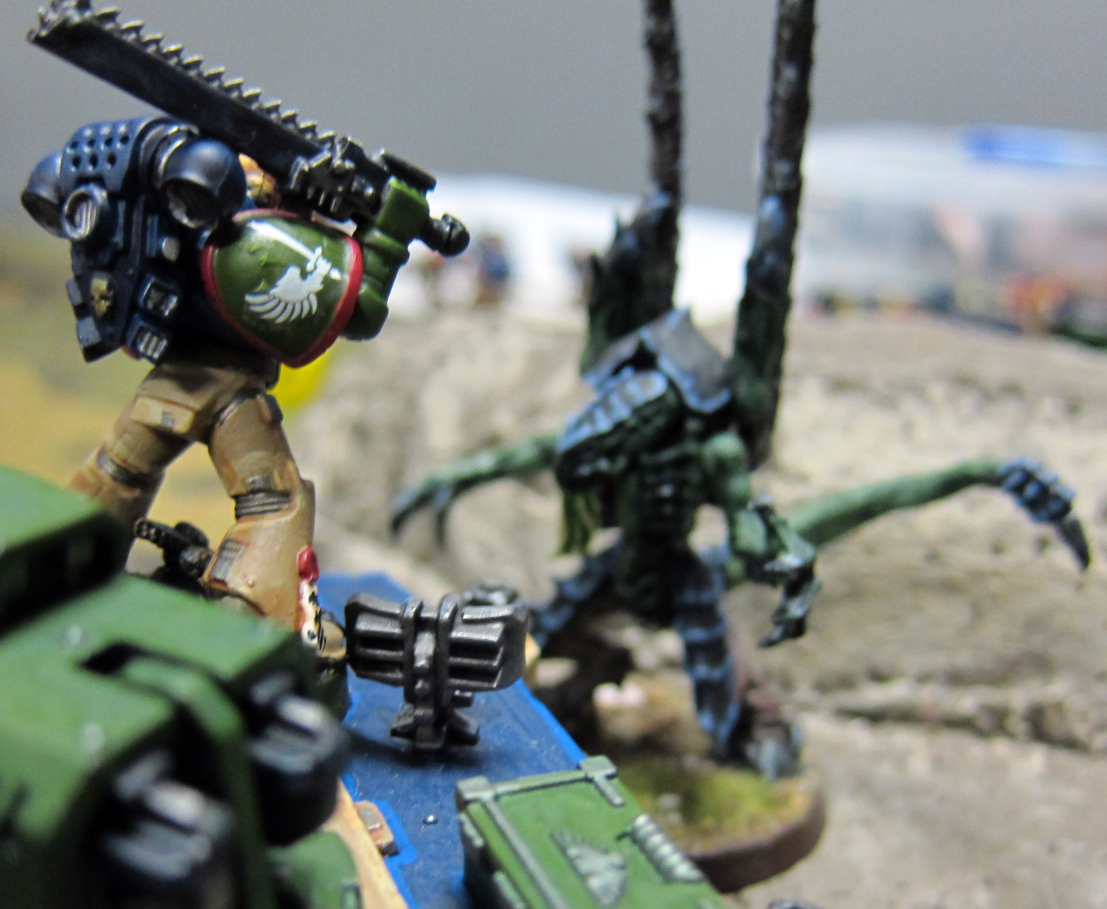
\includegraphics[width=(\linewidth-8pt)]{pics/titus-lictor-cropped}}\\
For the Emperor.
\end{minipage}
\vfill

\columnbreak

%%------------------------------------------------------
\missionheading{Traits}%

%Some models are given special roles and abilities.

\vspace{-9pt}%
\missionsubheading{Leader.} Each army's leader is its non-vehicle
model with highest leadership; designate one if several tie.

%\vspace{-9pt}%
\missionsubheading{Specialists.}  The leader and 3 other
non-vehicle models are also designated as specialists.  Each is given
a specialist trait from the following USRs, with no repetitions,
selected as part of the army list.

\vspace*{6pt}
\hrule
\noindent\begin{tabular*}{\linewidth}{>{\centering}p{0.5\linewidth} c}
  Acute Senses & Lance $^\dagger$ \\
  Adamantium Will & Master-Crafted $^\dagger$ \\
  Armourbane $^\dagger$ & Move Through Cover \\
  Blind $^\dagger$ & Night Vision \\
  Concussive $^\dagger$ & Pinning $^\dagger$ \\
  Counter-Attack & Poisoned (4+) $^\dagger$ \\
  Crusader & Preferred Enemy (All) \\
  Eternal Warrior & Rage \\
  Fear & Rampage \\
  Fearless & Relentless \\
  Feel No Pain & Rending $^\dagger$ \\
  Fleet & Scout \\
  Fleshbane $^\dagger$ & Shred $^\dagger$ \\
  Furious Charge & Shrouded \\
  Hammer of Wrath & Skilled Rider \\
  Hatred (All) & Sniper $^\dagger$ \\ 
  Haywire $^\dagger$ & Soul Blaze $^\dagger$ \\
  Hit \& Run & Stealth \\
  Ignores Cover & Strikedown $^\dagger$ \\
  Infiltrate & Stubborn \\
  Interceptor & Tank Hunter \\ 
\end{tabular*}

\smallskip
\centerline{$\dagger$ Designate 1 weapon to which the rule will apply.}
\hrule

\missionsubheading{Stratagem.}  Before either player deploys, each
simultaneously declares one of the following stratagems.

\begin{squishitemize}%
\item \emph{Just As Planned:} Seize the Initiative on a 4+.

\item \emph{Change Of Plans:} D3+2 non-vehicle models gain Scout (but
  still may not deploy in reserve).

\item \emph{Tactical Genius:} D3+2 non-vehicle models, and their
  dedicated transports if embarked, may deploy in reserve and gain
  Outflank.

%  Dedicated transports may be reserved with them, as usual.

% \item \emph{Tactical Genius:} D3+2 non-vehicle models may deploy in
%   reserve, ignoring No Holding Back (below), and gain Outflank.
%   Dedicated transports may be reserved with them, as usual.

\item \emph{We Came Here For You:} D3+2 non-vehicle models gain
  Preferred Enemy (All).

\item \emph{This Far, No Farther:} D3 models gain Fearless.

\item \emph{Hero Exemplar:} Units within~12'' of the leader may use
  its leadership for breaking point morale checks (below) if the
  leader passed its own.
\end{squishitemize}


%%------------------------------------------------------
\pagebreak
\missionheading{Setup and General Play}%

\vspace{-9pt}%
\missionsubheading{Army Of One.}  Before deployment, every model in
the player's army list is separated into individual units. This
includes models purchased as upgrades, such as Tau Drones. These
individual model units are deployed and play as normal units for all
game purposes. Unless specifically noted otherwise, the original army
list unit selections are not considered.

\missionsubheading{No Holding Back.}  Models may not be placed
into reserve unless specifically noted otherwise in the Recon Squad or
mission rules. All units that must start in reserve per their rules
but are not permitted to do so by these rules are deployed on the
table as any other unit. Units that enter ongoing reserves are removed
from the game and count as a casualty.

\missionsubheading{Help's Not Coming.}  No models beyond those in
the army lists may be added to the game in any way.

\missionsubheading{Side Effects.}  Rules conferred or applicable
to the models of an army list selection due to one model's special
rule or wargear are applicable to all the single model units created
from that selection when within~3'' of that model, or before
deployment.

%% Examples include Scout, Resurrection Orbs, Sgt Harker's Catachan
%% Devils, and Sgt Telion's Voice of Experience.

\missionheading{Movement Phase}%

\vspace{-9pt}%
\missionsubheading{We All Die Alone.}  At no point are independent
characters allowed to join units.

\missionsubheading{Get To The 'Choppa!}  Multiple units may embark
in a transport, up to its usual model capacity. Only independent
characters and units from the same original army list selection may
deploy embarked in a dedicated transport chosen with that selection.

\missionsubheading{Everyone Falls The First Time.}  Any model may
attempt to jump across gaps of up to~6'' between terrain.
Non-vehicles take an Initiative test with a~-1 penalty for each full
inch of gap after the first.  Vehicles take a dangerous terrain test
with the same penalty.  If successful the model may cross the gap but
otherwise moves as usual, i.e., must adhere to its distance limit.
Difficult terrain applies as well, based on the starting and ending
terrain, rolled before declaring a jump.

If the model fails, place it at the bottom of the gap in (base)
contact with the near edge.  It immediately suffers an automatic
Strength X hit, where X is the distance fallen in inches, rounding up.
If the distance is greater than~10 a Strength~10 hit is suffered but
no saves are allowed.  Vehicles are hit on their rear armor as well as
immobilized by the failed dangerous terrain test as usual.  The
vertical distance fallen does not count toward the model's movement,
and it may continue moving as usual if it survives and is able.

Any model may also jump down a vertical surface, applying the
preceding rules for a failed gap jump.

\missionheading{Psychic Phase}%

\vspace{-9pt}%
\missionsubheading{Cast A Spell On You.}  Each turn, a single
model from each original army list unit selection with the Brotherhood
of Psykers/Sorcerers rule may act as a Psyker (Mastery Level 1).  That
rule has no other effect.

\missionheading{Shooting and Assault Phases}%

\vspace{-9pt}%%
\missionsubheading{Unload.}  Shooting attacks with multiple shots may
be divided and allocated across multiple target units, provided each
target is within 3'' of the first.  This must be declared and done
before any rolls to hit or scatter.

\missionsubheading{Frag Bag.} A model may only make a shooting attack
with grenades once per game per such wargear item.

% \missionsubheading{Every Man Matters.}  All non-vehicle units are
% scoring unless specifically noted otherwise.  All units are denial
% units unless specifically noted otherwise.

%\missionheading{Assault Phase}%

\missionsubheading{Dogs Of War.}  Units may assault targets other than
those at which they shot.  All other restrictions apply.


\missionheading{Endgame}%

\vspace{-9pt}%
\missionsubheading{Boots On The Ground.} Vehicles and buildings are
not scoring units unless specifically noted so by mission rules.
Embarked scoring units may score objective markers, measuring from the
hull or main wall.

\missionsubheading{Breaking Point.}  From the start of the controlling
player's turn in which less than~50\% of its units remain, an army is
considered broken.  Before any other action, each of its units must
take a morale check, beginning with the leader.  Units within~6'' of
the leader may use its leadership for this if the leader passed.

\missionheading{Codex Specific Adaptations}%

\vspace{-9pt}%
\missionsubheading{Astra Militarum.} Orders are issued to a single
model unit and, if successful, applied to that model and all models
from the same army list selection within~3''.

\vspace{-9pt}%
\missionsubheading{Chaos Daemons and Space Marines.} The Warp Storm
and Champion of Chaos rules are not applied.

%\vspace{-9pt}%
%\missionsubheading{Chaos Daemons.} The Warp Storm is not applied.

%\vspace{-9pt}%
%\missionsubheading{Chaos Space Marines.} The 
%rule is not applied.

\vspace{-9pt}%
\missionsubheading{Dark Eldar.} Models with the Power from Pain
special rule earn one Pain Token for every~3 non-vehicle models they
have killed. Necron models only count after having failed their
Reanimation Protocols.

\vspace{-9pt}%
\missionsubheading{Necrons.} Necron models to be removed as casualties
are marked with a counter.  Reanimation Protocol rolls are made for
each such model within~6'' of a friendly Necron model, excluding other
casualties; otherwise reanimation fails automatically.  If successful
the model continues with~1 wound; otherwise it is removed.  Remove the
counter in either case.

\end{columns}

% \begin{story}{0.35in}{Unexpected Guests}%
%   Slowly, silently with his boot, Veteran Anders pushed more of the
%   burned planet's ubiquitous crumbly cinders up around his cook stove.
%   Ash swirled in the occasional stabbing wind as it stole the heat
%   from his dinner.  At the slightest crunch of rubble just out of
%   sight he instantly reached for his shotgun.  As far as he knew,
%   nobody friendly was anywhere near this post.
%\end{story}
